\chapter{METODOLOGI PENELITIAN}
Pada bagian ini peniliti menggunakan dua jenis data yaitu data primer dan data sekunder. Data primer adalah data yang diperoleh dari hasil kuisoner dan data sekunder yang diperoleh dari hasil penilitian sebelumnya.

\section{Data dan Pengumpulan Data}
Penulis menggunakan beberapa tahap atau metode dalam melakukan penilitian untuk menyusul proposal skripsi, yaitu :

\begin{enumerate}
    \item Studi Pustaka \\ Peneliti mengumpulkan data dengan cara mencari dari internet dan jurnal yang menyangkut atau jurnal yang membahas photon unity networking dalam pembuatan game multiplayer.
    \item Observasi \\ Peniliti mengumpulkan data dengan cara memainkan sekaligus mengamati secara langsung permainan sejenis yang sudah ada.
\end{enumerate}

\section{Rancangan Sistem(software/hardware)}
    Pada penilitian ini membutuhkan \textit{software} dan perangkat keras untuk melakukan pembuatan game first person shooter. Berikut ini spesifikasi rancangan sistem penilitian yang dijabarkan pada Tabel \ref{tb:tabel-spesifikasi}
    
    \begin{table}[h]
        \centering
        \begin{tabular}{|ll|lll}
        \cline{1-2}
        \multicolumn{2}{|c|}{Software}                                                &  &  &  \\ \cline{1-2}
        \multicolumn{1}{|l|}{Sistem Operasi} & Windows 11                             &  &  &  \\ \cline{1-2}
        \multicolumn{1}{|l|}{Tools}          & Unity 3D                                 &  &  &  \\ \cline{1-2}
        \multicolumn{2}{|c|}{Perangkat Keras}                                         &  &  &  \\ \cline{1-2}
        \multicolumn{1}{|l|}{Processor}      & Amd Ryzen 5 5400H With Radeon Graphics &  &  &  \\ \cline{1-2}
        \multicolumn{1}{|l|}{Memory}         & 8192MB Ram                             &  &  &  \\ \cline{1-2}
        \multicolumn{1}{|l|}{Video Card}     & Nvidia GeForce RTX 3050                &  &  &  \\ \cline{1-2}
        \multicolumn{1}{|l|}{SSD}            & 460GB                                  &  &  &  \\ \cline{1-2}
        \end{tabular}
        \caption{Tabel spesifikasi}
        \label{tb:tabel-spesifikasi}
        \end{table}

% \subsection{Rancangan Algoritma Matchmaking}
% Matchmaking dalam fitur permainan ini berperan sangat penting dan merupakan peran utama. Dalam peran tersebut, matchmaking mempertemukan antar pemain yang sedang aktif dalam melakukan pencarian room. Berikut penjelasan algoritma dalam bentuk \textit{flowchart} pada gambar 1.
% \begin{figure}[h]
%     \centering
%     \caption{Konteks  Algoritma Matchmaking}
%     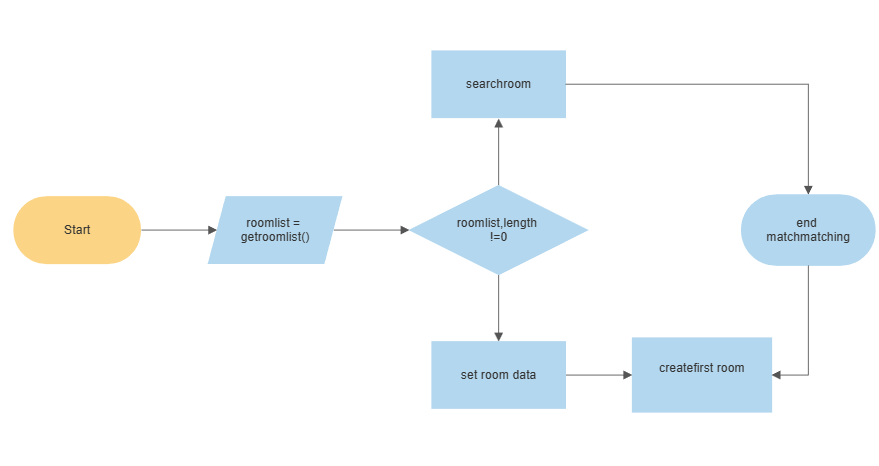
\includegraphics[width=15cm]{flowchart-matchmaking}
%     \label{fig:algoritmamatmaching}
%     \end{figure}


%     Mengacu pada gambar \ref{fig:algoritmamatmaching}, algoritma membutuhkan daftar \textit{room} yang didapatkan dari \textit{interface} photon \textit{Behavior}. Jika belum ada \textit{room} yang tersedia pada daftar \textit{room}, maka dilakukan fungsi detil dari algoritma matchmaking yaitu SearchRoomMatchmaking(). Berikut detil penjelasan flowchart pada gambar \ref{fig:detail-mm-1} dan gambar \ref{fig:detail-mm-2}.
%     \newpage
%     \begin{figure}[h]
%         \centering
%         \caption{Detail Algoritma Matchmaking 1}
%         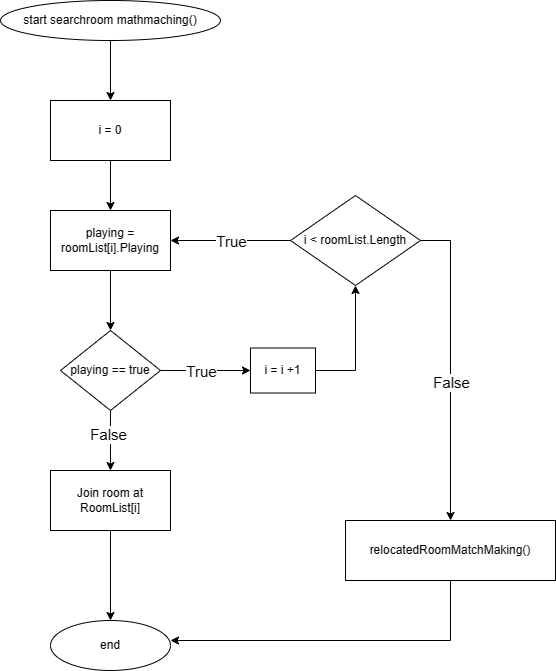
\includegraphics[width=10cm]{detail-algoritma-matmaking1.png}
%         \label{fig:detail-mm-1}
%         \end{figure}


%         Mengacu pada Gambar \ref{fig:detail-mm-1}, ketika fungsi ini dipanggil, 
% maka ia akan memulai perulangan sebanyak daftar room yang 
% tersedia. Pencarian bertujuan untuk mencari room yang memiliki 
% status sedang tidak bermain (waiting). Jika tidak menemukan 
% room yang tersedia dan ber-status tidak sedang bermain (waiting) 
% maka akan dilakukan pemanggilan fungsi 
% RealocateRoomMatchmaking() yang dijelaskan lebih detil pada 
% Gambar \ref{fig:detail-mm-2}. Jika sebaliknya maka pemain akan bergabung ke 
% dalam room.

% \newpage
% \begin{figure}[h]
%     \centering
%     \caption{Detail Algoritma Matchmaking 2}
%     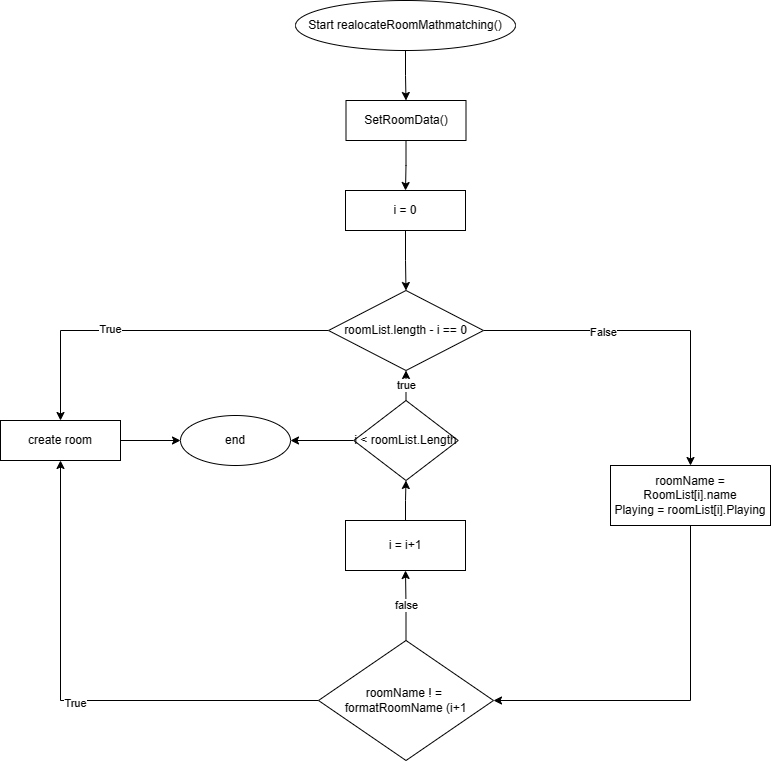
\includegraphics[width=10cm]{detail-algoritma-matmaking2.png}
%     \label{fig:detail-mm-2}
%     \end{figure}

\subsection{Use Case Diagram}
Tahapan ini memiliki satu aktor yaitu pemain, penjelasan mengenai tahap ini diilustrasikan pada gambar \ref{fig:case-diagram}

\begin{figure}[h]
    \centering
    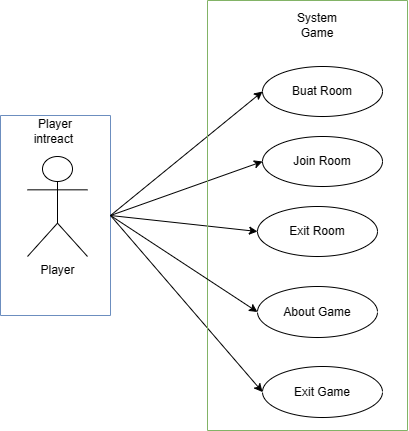
\includegraphics[width=10cm]{case-diagram.png}
    \caption{Use Case Diagram}
    \label{fig:case-diagram}
\end{figure}

    Gambar \ref{fig:case-diagram} menjelaskan tentang \textit{Use Case Diagram} dimana terdapat satu aktor yaitu pemain, serta 5 \textit{Use Case} yaitu \textit{Buat Room, Join Room, Exit Room, About Game, Exit Game}.
Pemain dapat menjadi server jika pemain melakukan \textit{use case} buat room dan pemain juga bisa menjadi client jika pemain menggunakan \textit{use case join room}, tetapi jika tidak adanya pemain yang menggunakan \textit{use case} buat room, maka \textit{use case} join room tidak dapat digunakan oleh pemain yang menjadi client.
\textit{use case exit room} dapat dilakukan oleh pemain yang menjadi server maupun menjadi client, dan hal itu akan menghapus sesi room yang sudah dibuat jika semua pemain menggunakan \textit{use case exit room}. \textit{Use case about game} dapat dilakukan oleh pemain untuk mengetahui tentang game yang dimainkan, dan yang terakhir jika pemain ingin meninggalkam game, pemain mengunakan \textit{Use case Exit Game.}
\subsection{Activity Diagram}
\textit{Activity diagram} adalah diagram yang memodelkan aliran aktivitas pada sistem
\begin{enumerate}
    \item \textit{Activity Player}
    \begin{figure}[h]
        \centering
        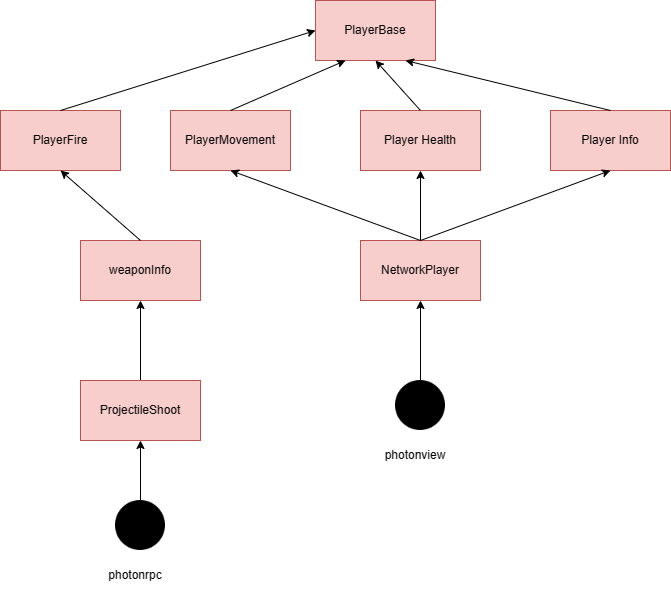
\includegraphics[width=10cm]{player-case.png}
        \caption{Activity Diagram Player}
        \label{fig:player-case}
    \end{figure}
    \\ Gambar \ref{fig:player-case} merupakan \textit{Activity Diagram Player}. Diawali dengan pemain harus terkoneksi jaringan photon, kemudian sistem akan memasuki ke layer network, yang akan menghubungkan beberapa komponen yaitu player movement, player health dan player info.
    Pada \textit{photon RPC} player memasuki ke sistem sinkronisasi kedalam \textit{projectileshoot} yang berfungsi disini sebagai menambak player musuh, kemudian memasukin activit weapon info yang berisi \textit{ammo weapon}, dan dari ammo yang tersedia mamsuki activity playerfire yang menandakan player siap memerangi player lain.
    \newpage
    \item \textit{Activity Diagram} buat \textit{Room}
     \begin{figure}[h]
        \centering
        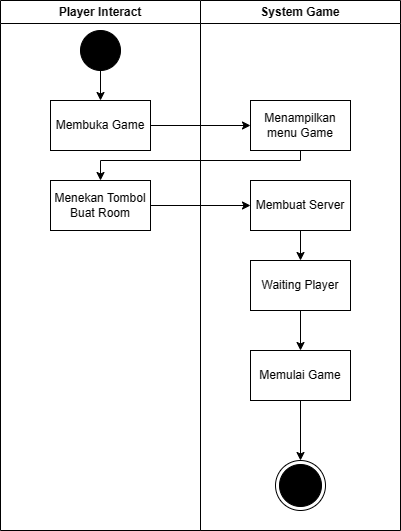
\includegraphics[width=10cm]{room-diagram.png}
        \caption{Activity Diagram Create Room}
        \label{fig:croom-case}
    \end{figure}
    \\ Gambar \ref{fig:croom-case} merupakan \textit{Activity Diagram Create Room}. Diawali dengan pemain membuka game, sistem akan menampilkan menu game, player menekan tombol buat room untuk membuat room yang belum tersedia sebagai server atau pemilk room.
    Pada \textit{activity waiting player} pemilik room akan menunggu player/\textit{client} untuk memasukan room dan memulai game.
    \newpage
    \item \textit{Activty Diagram} join \textit{Room}
    \begin{figure}[h]
        \centering
        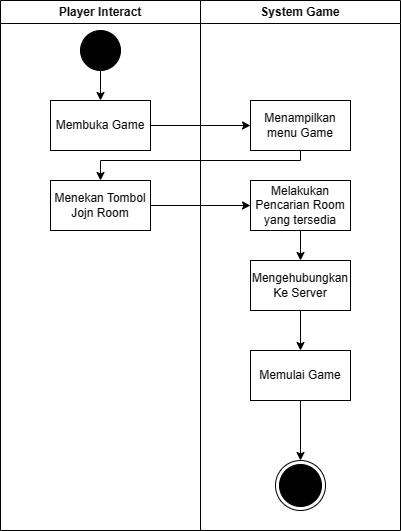
\includegraphics[width=10cm]{joinroom-diagram.png}
        \caption{Activity Diagram Join Room}
        \label{fig:jroom-case}
    \end{figure}
    \\ Gambar \ref{fig:jroom-case} merupakan \textit{activity diagram join room}. Diawali dengan pemain membuka game, kemudian sistem akan menampilkan menu dari game, player menekan tombol join room, photon unity akan mencarikan room yang tersedia yang sudah dibuat oleh pemain lain atau bisa mengetikan manual custom port yang terdapat pada pembuat room. Pemain akan terhubung ke server atau room yang tersedia jika room valid.
    \newpage
    \item  \textit{Activity Diagram Exit Room}
    \begin{figure}[h]
        \centering
        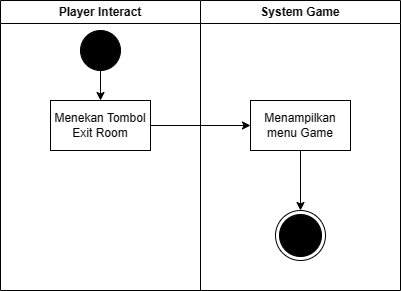
\includegraphics[width=10cm]{exitroom-diagram.png}
        \caption{Activity Diagram Exit Room}
        \label{fig:eroom-case}
    \end{figure}
    \\ Gambar \ref{fig:eroom-case} merupakan \textit{activity diagram exit room}. Diawali dengan pemain menekan tombol exit room, sistem akan menampilkan menu utama pada game.
    \item \textit{Activity Diagram About Room}
     \begin{figure}[h]
        \centering
        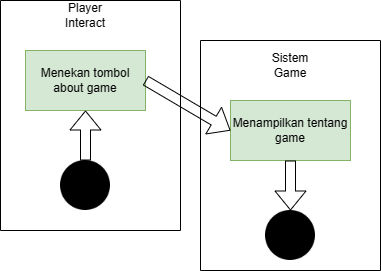
\includegraphics[width=10cm]{aboutcase-diagram.png}
        \caption{Activity Diagram About Room}
        \label{fig:aroom-case}
    \end{figure}
    \\ Gambar \ref{fig:aroom-case} merupakan \textit{activity diagram about room}. Diawali dengan pemain menekan tombol \textit{about room}. Sistem akan menampulkan isi tentang game yang dimainkan.
    \item  \textit{Activity Diagram Exit Game}
    \begin{figure}[h]
        \centering
        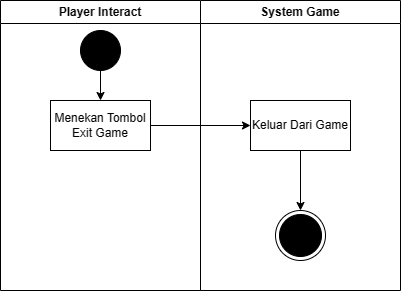
\includegraphics[width=10cm]{exitgame-diagram.png}
        \caption{Activity Diagram Exit Game}
        \label{fig:egame-case}
    \end{figure}
    \\ Gambar \ref{fig:egame-case} merupakan \textit{activity diagram exit game}. Diawali dengan pemain menekan tombol \textit{exit game}. Sistem akan mengeluarkan pemain dari game yang sedang dimainkan.
\end{enumerate}

% \subsection{Rancangan Arsitektur Umum Matchmaking}
% Photon memiliki fitur dan metode sendiri dalam mengelola sebuah \textit{game} multiplayer yang menggunakan \textit{framework}-nya.
% Photon Unity Networking merupakan class library yang dibungkus menjadi framework untuk mengelola pertukaran data sinkronisasi antar klien melalui Photon Cloud. 
% Arsitektur aplikasi permainan jak meuprang ini pada umumnya mempertemukan player pada lobby terlebih dahulu sebagai syarat memulai permainan dengan memanfaatkan event dan state yang ada pada Photon Unity Networking, komponen data pemain dan \textit{room} tersimpan dalam \textit{Custom Properties}. Berikut adalah arsitektur sistem dari aplikasi permainan pada Gambar \ref{fig:rumum-arsi}.
% \newpage
% \begin{figure}
%     \centering
%     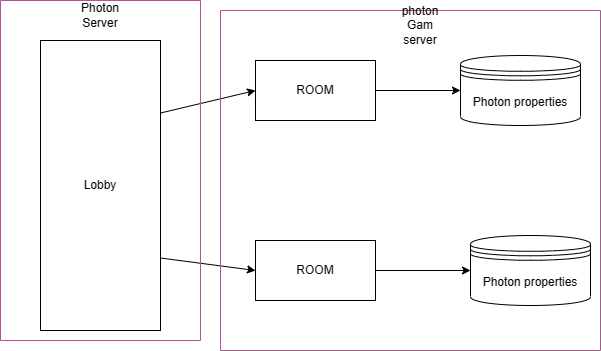
\includegraphics[width=10cm]{rancangan-arsitektur.png}
%     \caption{Rancangan Arsitektur Umum Matchmaking}
%     \label{fig:rumum-arsi}
% \end{figure}

\subsection{Class Diagram Network}
Rancangan kelas diagram ini merupakan bagian penting dari fitur \textit{Synchronous Multiplayer} dan akan diimplementasikan sesuai dengan rancangan diagram kelas seperti gambar \ref{fig:class-network}.

Pada kelas NetworkSpawner berfungsi untuk melakukan instansiasi objek karakter pemain dan menghidupkan kembali jika karakter pemain dalam keadaan \textit{state} mati.

Pada kelas NetworkMatchmaking, kelas ini akan menunggu event dari kelas NetworkManager. NetworkMatchmaking tidak dapat berjalan tanpa dikendalikan oleh NetworkManager.

Photon memiliki fitur penyimpanan \textit{state} sementara pada \textit{server}-nya (Photon Cloud), fitur tersebut berguna untuk menyimpan informasi \textit{room}, skor \textit{leaderboard} tiap pemain.
Fiture tersebut yaitu Photon Room Properties dan Photon Player Properties.
Perbedaanya adalah, penyimpanan dalam Photon Room Properties dapat diketahui nilainya oleh klien dalam satu \textit{room} yang sama, tetapi jika ingin mendapatkan nilai informasi dalam sebuah \textit{room} melalui Photon Room Properties, maka \textit{masterclient} diroom yang bersangkutan harus melakukan pengaturan pada \textit{method} CustomPropertiesForLobby yang terdapat pada photon.
Sedangkan Photon Player Properties hanya dapat diakses ketika dalam satu room yang sama.

NetworkPlayerProperty dan NetworkRoomProperty bertugas untuk menyimpan nilai \textit{unique} yang terdapat pada Photon Player Properties dan Photon Room Properties.

\begin{figure}[h]
    \centering
    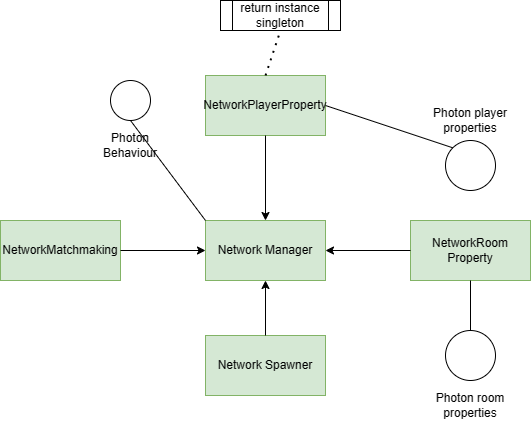
\includegraphics[width=8cm]{class-diagram-network.png}
    \caption{Class Diagram Network}
    \label{fig:class-network}
\end{figure}

\section{Metode dan Variabel Penelitian}
\subsection{Metode Penelitian}
Photon memiliki fitur dan metode sendiri dalam mengelola sebuah \textit{game} multiplayer yang menggunakan \textit{framework}-nya. Metode penelitian yang menggunakan framework photon unity dapat digambarkan ke dalam bentuk flowchart seperti gambar .
        \begin{figure}[h]
         \centering
         \caption{flowchart Algoritma Matchmaking}
         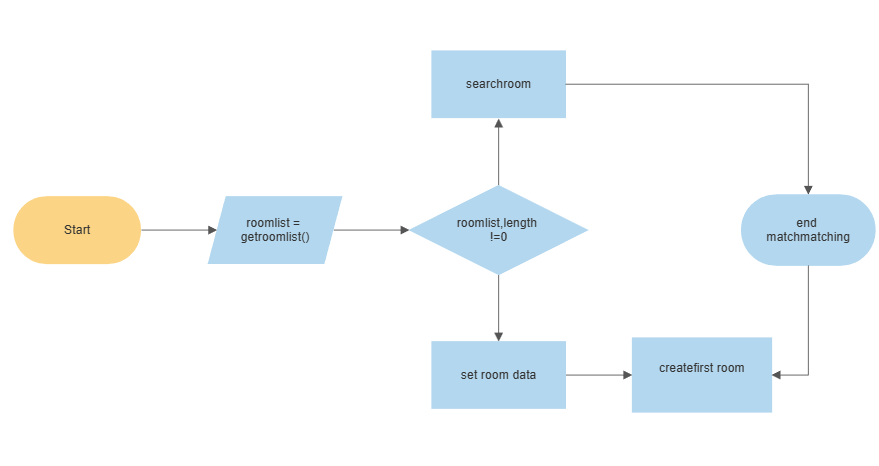
\includegraphics[width=10cm]{flowchart-matchmaking}
         \label{fig:algoritmamatmaching}
         \end{figure}

\newpage
Mengacu pada gambar \ref{fig:algoritmamatmaching}, algoritma membutuhkan daftar \textit{room} yang didapatkan dari \textit{interface} photon \textit{Behavior}. Jika belum ada \textit{room} yang tersedia pada daftar \textit{room}, maka dilakukan fungsi detil dari algoritma matchmaking yaitu SearchRoomMatchmaking(). 

% Berikut detil penjelasan flowchart pada gambar \ref{fig:detail-mm-1} dan gambar \ref{fig:detail-mm-2}.
% \begin{figure}[h]
%             \centering
%             \caption{Detail Algoritma Matchmaking 1}
%             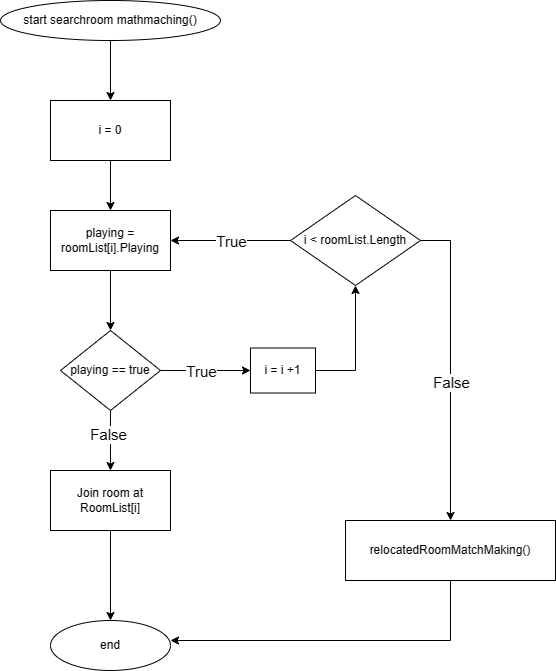
\includegraphics[width=10cm]{detail-algoritma-matmaking1.png}
%             \label{fig:detail-mm-1}
%             \end{figure}
    
    
%             Mengacu pada Gambar \ref{fig:detail-mm-1}, ketika fungsi ini dipanggil, 
%     maka ia akan memulai perulangan sebanyak daftar room yang 
%     tersedia. Pencarian bertujuan untuk mencari room yang memiliki 
%     status sedang tidak bermain (waiting). Jika tidak menemukan 
%     room yang tersedia dan ber-status tidak sedang bermain (waiting) 
%     maka akan dilakukan pemanggilan fungsi 
%     RealocateRoomMatchmaking() yang dijelaskan lebih detil pada 
%     Gambar \ref{fig:detail-mm-2}. Jika sebaliknya maka pemain akan bergabung ke 
%     dalam room.
    
%     \newpage
%     \begin{figure}[h]
%         \centering
%         \caption{Detail Algoritma Matchmaking 2}
%         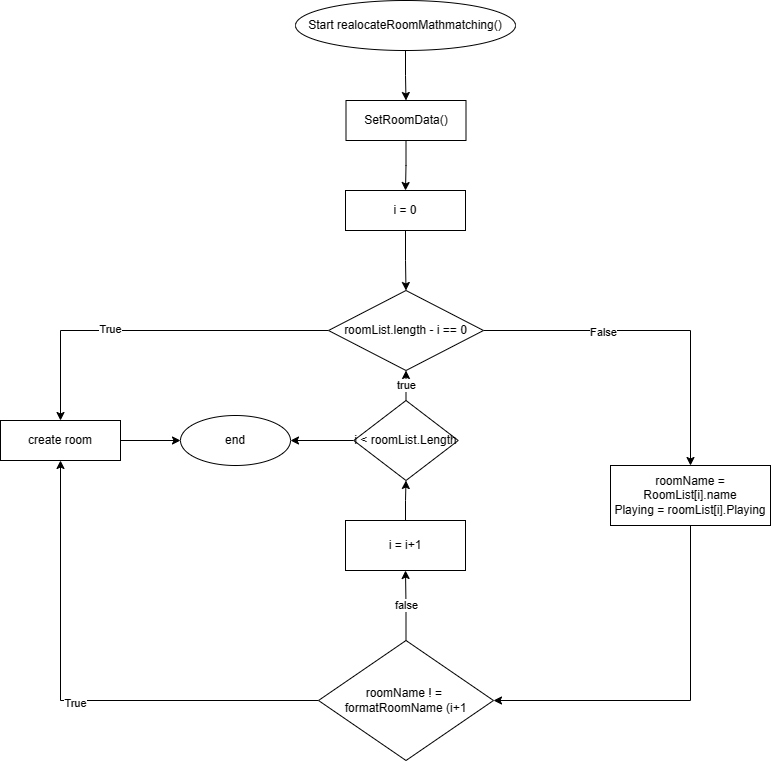
\includegraphics[width=10cm]{detail-algoritma-matmaking2.png}
%         \label{fig:detail-mm-2}
%         \end{figure}

        \subsection{Variabel Penelitian}

        Variabel yang digunakan dalam penelitian ini yaitu berupa framework unity menggunakan Photon Unity Networking yang berguna untuk mengelola pertukaran data sinronisasi antara klien melalui photon cloud untuk menjumpai sesama player pada room didalam aplikasi permainan.

        \section{Teknik Pengujian}
\subsection{Pengujian \textit{Black Box}}
Pengujian Black Box pada fungsional sistem yang terdapat pada aplikasi permainan jak meuprang.

    \begin{table}[h]
    \centering
    \begin{tabular}{|l|l|l|l|}
    \hline
    \multicolumn{1}{|c|}{NO} & \multicolumn{1}{c|}{Aktivitas Pengujian} & \multicolumn{1}{c|}{Hasil yang diharapkan} & \multicolumn{1}{c|}{Kesimpulan} \\ \hline
    1                        & Tombol Buat Room                         & Membuka panel "Room Panel"                 &                                 \\ \hline
    2                        & Tombol Join Room                         & Membuka panel "Lobby Panel"                &                                 \\ \hline
    3                        & Tombol Exit Room                         & Kembali ke menu utama                      &                                 \\ \hline
    4                        & Tombol About Game                        & Menampilkan popup about game               &                                 \\ \hline
    5                        & Tombol exit game                         & Keluar dari aplikasi game                  &                                 \\ \hline
    \end{tabular}
    \caption{Tabel Pengujian Black Box}
    \label{lab:tabel-pengujian}
    \end{table}
        
\section{Hasil yang diharapkan}
Hasil yang diharapkan pada penilitian ini antara lain :
\begin{enumerate}
    \item Keberhasilan dalam mengetahui kelayakan aplikasi game dengan metode \textit{blackbox testing}.
    \item Keberhasilan game terhubung dengan unity python networking yang dapat dimainkan secara multiplayer online.
    \item Laporan tugas akhir mahasiswa jurusan Teknologi Informasi Dan Komputer.
\end{enumerate}